% Created by tikzDevice version 0.12.3.1 on 2021-12-08 12:30:27
% !TEX encoding = UTF-8 Unicode
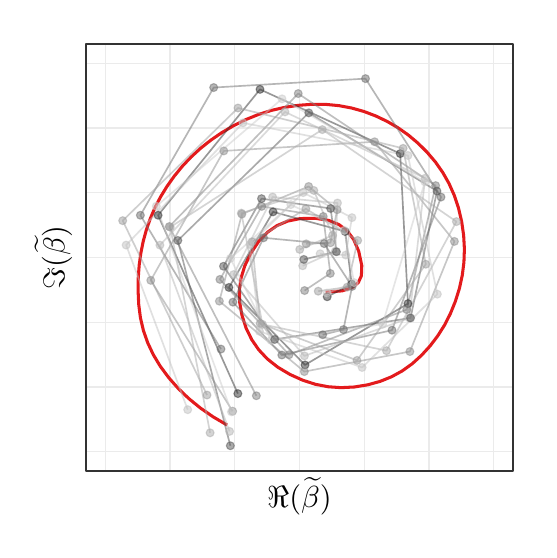
\begin{tikzpicture}[x=1pt,y=1pt]
\definecolor{fillColor}{RGB}{255,255,255}
\begin{scope}
\definecolor{drawColor}{RGB}{255,255,255}
\definecolor{fillColor}{RGB}{255,255,255}

\path[draw=drawColor,line width= 0.6pt,line join=round,line cap=round,fill=fillColor] (  0.00,  0.00) rectangle (180.67,180.68);
\end{scope}
\begin{scope}
\definecolor{fillColor}{RGB}{255,255,255}

\path[fill=fillColor] ( 20.71, 20.71) rectangle (175.17,175.17);
\definecolor{drawColor}{gray}{0.92}

\path[draw=drawColor,line width= 0.3pt,line join=round] ( 20.71, 27.74) --
	(175.17, 27.74);

\path[draw=drawColor,line width= 0.3pt,line join=round] ( 20.71, 74.54) --
	(175.17, 74.54);

\path[draw=drawColor,line width= 0.3pt,line join=round] ( 20.71,121.35) --
	(175.17,121.35);

\path[draw=drawColor,line width= 0.3pt,line join=round] ( 20.71,168.15) --
	(175.17,168.15);

\path[draw=drawColor,line width= 0.3pt,line join=round] ( 27.74, 20.71) --
	( 27.74,175.17);

\path[draw=drawColor,line width= 0.3pt,line join=round] ( 74.54, 20.71) --
	( 74.54,175.17);

\path[draw=drawColor,line width= 0.3pt,line join=round] (121.35, 20.71) --
	(121.35,175.17);

\path[draw=drawColor,line width= 0.3pt,line join=round] (168.15, 20.71) --
	(168.15,175.17);

\path[draw=drawColor,line width= 0.6pt,line join=round] ( 20.71, 51.14) --
	(175.17, 51.14);

\path[draw=drawColor,line width= 0.6pt,line join=round] ( 20.71, 97.94) --
	(175.17, 97.94);

\path[draw=drawColor,line width= 0.6pt,line join=round] ( 20.71,144.75) --
	(175.17,144.75);

\path[draw=drawColor,line width= 0.6pt,line join=round] ( 51.14, 20.71) --
	( 51.14,175.17);

\path[draw=drawColor,line width= 0.6pt,line join=round] ( 97.94, 20.71) --
	( 97.94,175.17);

\path[draw=drawColor,line width= 0.6pt,line join=round] (144.75, 20.71) --
	(144.75,175.17);
\definecolor{drawColor}{RGB}{227,26,28}

\path[draw=drawColor,line width= 1.1pt,line join=round] (107.35, 85.39) --
	(113.40, 85.89) --
	(117.08, 87.13) --
	(119.19, 88.89) --
	(120.29, 91.34) --
	(120.43, 95.02) --
	(119.31,100.23) --
	(117.47,104.49) --
	(115.13,107.59) --
	(112.20,109.82) --
	(108.46,111.34) --
	(103.59,112.10) --
	( 98.25,112.00) --
	( 93.72,111.11) --
	( 89.82,109.47) --
	( 86.35,107.06) --
	( 83.18,103.75) --
	( 80.29, 99.41) --
	( 78.16, 94.93) --
	( 76.82, 90.56) --
	( 76.21, 86.20) --
	( 76.30, 81.75) --
	( 77.12, 77.08) --
	( 78.64, 72.39) --
	( 80.66, 68.26) --
	( 83.19, 64.59) --
	( 86.27, 61.31) --
	( 90.00, 58.35) --
	( 94.45, 55.69) --
	( 99.09, 53.59) --
	(103.68, 52.11) --
	(108.27, 51.23) --
	(112.93, 50.90) --
	(117.74, 51.14) --
	(122.60, 51.93) --
	(127.07, 53.17) --
	(131.20, 54.84) --
	(135.03, 56.94) --
	(138.63, 59.52) --
	(142.03, 62.60) --
	(145.14, 66.01) --
	(147.89, 69.63) --
	(150.32, 73.49) --
	(152.43, 77.62) --
	(154.23, 82.05) --
	(155.71, 86.77) --
	(156.74, 91.50) --
	(157.34, 96.24) --
	(157.51,101.02) --
	(157.24,105.90) --
	(156.52,110.90) --
	(155.38,115.79) --
	(153.87,120.35) --
	(151.98,124.61) --
	(149.71,128.62) --
	(147.05,132.42) --
	(143.98,136.03) --
	(140.69,139.29) --
	(137.23,142.20) --
	(133.56,144.79) --
	(129.67,147.07) --
	(125.51,149.06) --
	(121.17,150.71) --
	(116.74,151.95) --
	(112.20,152.80) --
	(107.52,153.25) --
	(102.64,153.30) --
	( 97.57,152.93) --
	( 92.60,152.19) --
	( 87.80,151.09) --
	( 83.15,149.63) --
	( 78.61,147.80) --
	( 74.15,145.59) --
	( 69.84,143.05) --
	( 65.85,140.31) --
	( 62.15,137.37) --
	( 58.73,134.23) --
	( 55.57,130.88) --
	( 52.64,127.29) --
	( 50.02,123.59) --
	( 47.72,119.84) --
	( 45.73,116.01) --
	( 44.04,112.09) --
	( 42.62,108.05) --
	( 41.48,103.89) --
	( 40.61, 99.62) --
	( 40.00, 95.22) --
	( 39.66, 90.66) --
	( 39.60, 85.92) --
	( 39.82, 81.00) --
	( 40.44, 76.16) --
	( 41.52, 71.55) --
	( 43.07, 67.12) --
	( 45.09, 62.82) --
	( 47.63, 58.61) --
	( 50.68, 54.49) --
	( 54.10, 50.62) --
	( 57.88, 46.99) --
	( 62.06, 43.58) --
	( 66.67, 40.38) --
	( 71.76, 37.39);
\definecolor{drawColor}{RGB}{51,51,51}

\path[draw=drawColor,draw opacity=0.50,line width= 0.6pt,line join=round] (107.93, 83.74) --
	(116.78, 88.32) --
	(114.42,107.33) --
	( 88.37,114.42) --
	( 72.42, 87.11) --
	( 99.92, 59.10) --
	(137.11, 81.27) --
	(134.31,135.47) --
	( 83.65,158.68) --
	( 46.82,113.20) --
	( 75.65, 48.76);
\definecolor{drawColor}{RGB}{87,87,87}

\path[draw=drawColor,draw opacity=0.50,line width= 0.6pt,line join=round] ( 99.48, 97.23) --
	(111.27,100.01) --
	(109.17,115.64) --
	( 84.20,119.20) --
	( 70.46, 94.77) --
	( 88.96, 68.31) --
	(138.06, 76.08) --
	(147.60,121.94) --
	(101.28,150.20) --
	( 53.97,104.09) --
	( 72.93, 29.91);
\definecolor{drawColor}{RGB}{110,110,110}

\path[draw=drawColor,draw opacity=0.50,line width= 0.6pt,line join=round] (106.30, 70.02) --
	(113.81, 71.89) --
	(116.92, 87.48) --
	(106.83,102.95) --
	( 84.94,105.05) --
	( 73.87, 81.80) --
	( 91.54, 62.69) --
	(131.35, 71.67) --
	(149.06,119.77) --
	(121.77,162.57) --
	( 66.92,159.34) --
	( 40.43,113.20) --
	( 69.55, 64.84);
\definecolor{drawColor}{RGB}{129,129,129}

\path[draw=drawColor,draw opacity=0.50,line width= 0.6pt,line join=round] ( 99.77, 85.99) --
	(109.05, 92.18) --
	(106.50,112.76) --
	( 84.30,116.41) --
	( 69.17, 90.01) --
	( 94.14, 62.80) --
	(136.69, 79.10) --
	(147.12,123.91) --
	( 97.46,157.17) --
	( 50.87,109.10) --
	( 82.33, 47.97);
\definecolor{drawColor}{RGB}{145,145,145}

\path[draw=drawColor,draw opacity=0.50,line width= 0.6pt,line join=round] (100.34,102.85) --
	(109.12,103.25) --
	(111.54,115.19) --
	(101.24,123.59) --
	( 77.11,113.61) --
	( 68.97, 82.16) --
	( 99.67, 56.71) --
	(137.82, 63.94) --
	(153.90,103.74) --
	(125.05,139.75) --
	( 70.57,136.44) --
	( 44.18, 89.67) --
	( 73.76, 42.39);
\definecolor{drawColor}{RGB}{159,159,159}

\path[draw=drawColor,draw opacity=0.50,line width= 0.6pt,line join=round] (104.69, 85.76) --
	(115.15, 87.22) --
	(118.94,104.09) --
	(100.22,115.53) --
	( 80.78,103.62) --
	( 83.69, 74.08) --
	(118.71, 60.75) --
	(143.56, 95.50) --
	(135.36,137.37) --
	( 75.69,151.95) --
	( 34.04,111.24) --
	( 64.50, 48.24);
\definecolor{drawColor}{RGB}{171,171,171}

\path[draw=drawColor,draw opacity=0.50,line width= 0.6pt,line join=round] ( 98.01,100.84) --
	(109.87,105.93) --
	(103.11,122.15) --
	( 76.92,113.96) --
	( 84.53, 73.78) --
	(129.36, 64.26) --
	(154.63,110.90) --
	(106.16,144.15) --
	( 51.23,108.90) --
	( 65.62, 34.58);
\definecolor{drawColor}{RGB}{183,183,183}

\path[draw=drawColor,draw opacity=0.50,line width= 0.6pt,line join=round] ( 99.07, 94.94) --
	(110.88,100.22) --
	(111.65,117.62) --
	( 88.21,119.79) --
	( 74.10, 91.76) --
	( 99.71, 62.38) --
	(137.62, 76.07) --
	(143.32,126.56) --
	( 92.68,150.54) --
	( 47.49,102.40) --
	( 72.65, 35.10);
\definecolor{drawColor}{RGB}{194,194,194}

\path[draw=drawColor,draw opacity=0.50,line width= 0.6pt,line join=round] (105.38, 99.29) --
	(114.63, 98.82) --
	(116.88,112.33) --
	( 99.27,121.38) --
	( 80.02,102.65) --
	( 83.47, 71.27) --
	(120.55, 58.20) --
	(147.73, 84.68) --
	(137.10,134.79) --
	( 77.50,146.58) --
	( 35.28,102.42) --
	( 57.53, 42.94);
\definecolor{drawColor}{RGB}{204,204,204}

\path[draw=drawColor,draw opacity=0.50,line width= 0.6pt,line join=round] (107.89, 85.09) --
	(117.66, 88.86) --
	(114.08,107.74) --
	( 94.79,117.04) --
	( 72.97, 97.61) --
	( 87.68, 68.01) --
	(127.95, 73.84) --
	(143.22,125.29) --
	( 91.61,155.26) --
	( 46.19,116.47) --
	( 73.32, 42.17);
\definecolor{drawColor}{RGB}{51,51,51}
\definecolor{fillColor}{RGB}{51,51,51}

\path[draw=drawColor,draw opacity=0.50,line width= 0.4pt,line join=round,line cap=round,fill=fillColor,fill opacity=0.50] (107.93, 83.74) circle (  1.43);

\path[draw=drawColor,draw opacity=0.50,line width= 0.4pt,line join=round,line cap=round,fill=fillColor,fill opacity=0.50] (116.78, 88.32) circle (  1.43);

\path[draw=drawColor,draw opacity=0.50,line width= 0.4pt,line join=round,line cap=round,fill=fillColor,fill opacity=0.50] (114.42,107.33) circle (  1.43);

\path[draw=drawColor,draw opacity=0.50,line width= 0.4pt,line join=round,line cap=round,fill=fillColor,fill opacity=0.50] ( 88.37,114.42) circle (  1.43);

\path[draw=drawColor,draw opacity=0.50,line width= 0.4pt,line join=round,line cap=round,fill=fillColor,fill opacity=0.50] ( 72.42, 87.11) circle (  1.43);

\path[draw=drawColor,draw opacity=0.50,line width= 0.4pt,line join=round,line cap=round,fill=fillColor,fill opacity=0.50] ( 99.92, 59.10) circle (  1.43);

\path[draw=drawColor,draw opacity=0.50,line width= 0.4pt,line join=round,line cap=round,fill=fillColor,fill opacity=0.50] (137.11, 81.27) circle (  1.43);

\path[draw=drawColor,draw opacity=0.50,line width= 0.4pt,line join=round,line cap=round,fill=fillColor,fill opacity=0.50] (134.31,135.47) circle (  1.43);

\path[draw=drawColor,draw opacity=0.50,line width= 0.4pt,line join=round,line cap=round,fill=fillColor,fill opacity=0.50] ( 83.65,158.68) circle (  1.43);

\path[draw=drawColor,draw opacity=0.50,line width= 0.4pt,line join=round,line cap=round,fill=fillColor,fill opacity=0.50] ( 46.82,113.20) circle (  1.43);

\path[draw=drawColor,draw opacity=0.50,line width= 0.4pt,line join=round,line cap=round,fill=fillColor,fill opacity=0.50] ( 75.65, 48.76) circle (  1.43);
\definecolor{drawColor}{RGB}{110,110,110}
\definecolor{fillColor}{RGB}{110,110,110}

\path[draw=drawColor,draw opacity=0.50,line width= 0.4pt,line join=round,line cap=round,fill=fillColor,fill opacity=0.50] (106.30, 70.02) circle (  1.43);

\path[draw=drawColor,draw opacity=0.50,line width= 0.4pt,line join=round,line cap=round,fill=fillColor,fill opacity=0.50] (113.81, 71.89) circle (  1.43);

\path[draw=drawColor,draw opacity=0.50,line width= 0.4pt,line join=round,line cap=round,fill=fillColor,fill opacity=0.50] (116.92, 87.48) circle (  1.43);

\path[draw=drawColor,draw opacity=0.50,line width= 0.4pt,line join=round,line cap=round,fill=fillColor,fill opacity=0.50] (106.83,102.95) circle (  1.43);

\path[draw=drawColor,draw opacity=0.50,line width= 0.4pt,line join=round,line cap=round,fill=fillColor,fill opacity=0.50] ( 84.94,105.05) circle (  1.43);

\path[draw=drawColor,draw opacity=0.50,line width= 0.4pt,line join=round,line cap=round,fill=fillColor,fill opacity=0.50] ( 73.87, 81.80) circle (  1.43);

\path[draw=drawColor,draw opacity=0.50,line width= 0.4pt,line join=round,line cap=round,fill=fillColor,fill opacity=0.50] ( 91.54, 62.69) circle (  1.43);

\path[draw=drawColor,draw opacity=0.50,line width= 0.4pt,line join=round,line cap=round,fill=fillColor,fill opacity=0.50] (131.35, 71.67) circle (  1.43);

\path[draw=drawColor,draw opacity=0.50,line width= 0.4pt,line join=round,line cap=round,fill=fillColor,fill opacity=0.50] (149.06,119.77) circle (  1.43);

\path[draw=drawColor,draw opacity=0.50,line width= 0.4pt,line join=round,line cap=round,fill=fillColor,fill opacity=0.50] (121.77,162.57) circle (  1.43);

\path[draw=drawColor,draw opacity=0.50,line width= 0.4pt,line join=round,line cap=round,fill=fillColor,fill opacity=0.50] ( 66.92,159.34) circle (  1.43);

\path[draw=drawColor,draw opacity=0.50,line width= 0.4pt,line join=round,line cap=round,fill=fillColor,fill opacity=0.50] ( 40.43,113.20) circle (  1.43);

\path[draw=drawColor,draw opacity=0.50,line width= 0.4pt,line join=round,line cap=round,fill=fillColor,fill opacity=0.50] ( 69.55, 64.84) circle (  1.43);
\definecolor{drawColor}{RGB}{129,129,129}
\definecolor{fillColor}{RGB}{129,129,129}

\path[draw=drawColor,draw opacity=0.50,line width= 0.4pt,line join=round,line cap=round,fill=fillColor,fill opacity=0.50] ( 99.77, 85.99) circle (  1.43);

\path[draw=drawColor,draw opacity=0.50,line width= 0.4pt,line join=round,line cap=round,fill=fillColor,fill opacity=0.50] (109.05, 92.18) circle (  1.43);

\path[draw=drawColor,draw opacity=0.50,line width= 0.4pt,line join=round,line cap=round,fill=fillColor,fill opacity=0.50] (106.50,112.76) circle (  1.43);

\path[draw=drawColor,draw opacity=0.50,line width= 0.4pt,line join=round,line cap=round,fill=fillColor,fill opacity=0.50] ( 84.30,116.41) circle (  1.43);

\path[draw=drawColor,draw opacity=0.50,line width= 0.4pt,line join=round,line cap=round,fill=fillColor,fill opacity=0.50] ( 69.17, 90.01) circle (  1.43);

\path[draw=drawColor,draw opacity=0.50,line width= 0.4pt,line join=round,line cap=round,fill=fillColor,fill opacity=0.50] ( 94.14, 62.80) circle (  1.43);

\path[draw=drawColor,draw opacity=0.50,line width= 0.4pt,line join=round,line cap=round,fill=fillColor,fill opacity=0.50] (136.69, 79.10) circle (  1.43);

\path[draw=drawColor,draw opacity=0.50,line width= 0.4pt,line join=round,line cap=round,fill=fillColor,fill opacity=0.50] (147.12,123.91) circle (  1.43);

\path[draw=drawColor,draw opacity=0.50,line width= 0.4pt,line join=round,line cap=round,fill=fillColor,fill opacity=0.50] ( 97.46,157.17) circle (  1.43);

\path[draw=drawColor,draw opacity=0.50,line width= 0.4pt,line join=round,line cap=round,fill=fillColor,fill opacity=0.50] ( 50.87,109.10) circle (  1.43);

\path[draw=drawColor,draw opacity=0.50,line width= 0.4pt,line join=round,line cap=round,fill=fillColor,fill opacity=0.50] ( 82.33, 47.97) circle (  1.43);
\definecolor{drawColor}{RGB}{145,145,145}
\definecolor{fillColor}{RGB}{145,145,145}

\path[draw=drawColor,draw opacity=0.50,line width= 0.4pt,line join=round,line cap=round,fill=fillColor,fill opacity=0.50] (100.34,102.85) circle (  1.43);

\path[draw=drawColor,draw opacity=0.50,line width= 0.4pt,line join=round,line cap=round,fill=fillColor,fill opacity=0.50] (109.12,103.25) circle (  1.43);

\path[draw=drawColor,draw opacity=0.50,line width= 0.4pt,line join=round,line cap=round,fill=fillColor,fill opacity=0.50] (111.54,115.19) circle (  1.43);

\path[draw=drawColor,draw opacity=0.50,line width= 0.4pt,line join=round,line cap=round,fill=fillColor,fill opacity=0.50] (101.24,123.59) circle (  1.43);

\path[draw=drawColor,draw opacity=0.50,line width= 0.4pt,line join=round,line cap=round,fill=fillColor,fill opacity=0.50] ( 77.11,113.61) circle (  1.43);

\path[draw=drawColor,draw opacity=0.50,line width= 0.4pt,line join=round,line cap=round,fill=fillColor,fill opacity=0.50] ( 68.97, 82.16) circle (  1.43);

\path[draw=drawColor,draw opacity=0.50,line width= 0.4pt,line join=round,line cap=round,fill=fillColor,fill opacity=0.50] ( 99.67, 56.71) circle (  1.43);

\path[draw=drawColor,draw opacity=0.50,line width= 0.4pt,line join=round,line cap=round,fill=fillColor,fill opacity=0.50] (137.82, 63.94) circle (  1.43);

\path[draw=drawColor,draw opacity=0.50,line width= 0.4pt,line join=round,line cap=round,fill=fillColor,fill opacity=0.50] (153.90,103.74) circle (  1.43);

\path[draw=drawColor,draw opacity=0.50,line width= 0.4pt,line join=round,line cap=round,fill=fillColor,fill opacity=0.50] (125.05,139.75) circle (  1.43);

\path[draw=drawColor,draw opacity=0.50,line width= 0.4pt,line join=round,line cap=round,fill=fillColor,fill opacity=0.50] ( 70.57,136.44) circle (  1.43);

\path[draw=drawColor,draw opacity=0.50,line width= 0.4pt,line join=round,line cap=round,fill=fillColor,fill opacity=0.50] ( 44.18, 89.67) circle (  1.43);

\path[draw=drawColor,draw opacity=0.50,line width= 0.4pt,line join=round,line cap=round,fill=fillColor,fill opacity=0.50] ( 73.76, 42.39) circle (  1.43);
\definecolor{drawColor}{RGB}{159,159,159}
\definecolor{fillColor}{RGB}{159,159,159}

\path[draw=drawColor,draw opacity=0.50,line width= 0.4pt,line join=round,line cap=round,fill=fillColor,fill opacity=0.50] (104.69, 85.76) circle (  1.43);

\path[draw=drawColor,draw opacity=0.50,line width= 0.4pt,line join=round,line cap=round,fill=fillColor,fill opacity=0.50] (115.15, 87.22) circle (  1.43);

\path[draw=drawColor,draw opacity=0.50,line width= 0.4pt,line join=round,line cap=round,fill=fillColor,fill opacity=0.50] (118.94,104.09) circle (  1.43);

\path[draw=drawColor,draw opacity=0.50,line width= 0.4pt,line join=round,line cap=round,fill=fillColor,fill opacity=0.50] (100.22,115.53) circle (  1.43);

\path[draw=drawColor,draw opacity=0.50,line width= 0.4pt,line join=round,line cap=round,fill=fillColor,fill opacity=0.50] ( 80.78,103.62) circle (  1.43);

\path[draw=drawColor,draw opacity=0.50,line width= 0.4pt,line join=round,line cap=round,fill=fillColor,fill opacity=0.50] ( 83.69, 74.08) circle (  1.43);

\path[draw=drawColor,draw opacity=0.50,line width= 0.4pt,line join=round,line cap=round,fill=fillColor,fill opacity=0.50] (118.71, 60.75) circle (  1.43);

\path[draw=drawColor,draw opacity=0.50,line width= 0.4pt,line join=round,line cap=round,fill=fillColor,fill opacity=0.50] (143.56, 95.50) circle (  1.43);

\path[draw=drawColor,draw opacity=0.50,line width= 0.4pt,line join=round,line cap=round,fill=fillColor,fill opacity=0.50] (135.36,137.37) circle (  1.43);

\path[draw=drawColor,draw opacity=0.50,line width= 0.4pt,line join=round,line cap=round,fill=fillColor,fill opacity=0.50] ( 75.69,151.95) circle (  1.43);

\path[draw=drawColor,draw opacity=0.50,line width= 0.4pt,line join=round,line cap=round,fill=fillColor,fill opacity=0.50] ( 34.04,111.24) circle (  1.43);

\path[draw=drawColor,draw opacity=0.50,line width= 0.4pt,line join=round,line cap=round,fill=fillColor,fill opacity=0.50] ( 64.50, 48.24) circle (  1.43);
\definecolor{drawColor}{RGB}{171,171,171}
\definecolor{fillColor}{RGB}{171,171,171}

\path[draw=drawColor,draw opacity=0.50,line width= 0.4pt,line join=round,line cap=round,fill=fillColor,fill opacity=0.50] ( 98.01,100.84) circle (  1.43);

\path[draw=drawColor,draw opacity=0.50,line width= 0.4pt,line join=round,line cap=round,fill=fillColor,fill opacity=0.50] (109.87,105.93) circle (  1.43);

\path[draw=drawColor,draw opacity=0.50,line width= 0.4pt,line join=round,line cap=round,fill=fillColor,fill opacity=0.50] (103.11,122.15) circle (  1.43);

\path[draw=drawColor,draw opacity=0.50,line width= 0.4pt,line join=round,line cap=round,fill=fillColor,fill opacity=0.50] ( 76.92,113.96) circle (  1.43);

\path[draw=drawColor,draw opacity=0.50,line width= 0.4pt,line join=round,line cap=round,fill=fillColor,fill opacity=0.50] ( 84.53, 73.78) circle (  1.43);

\path[draw=drawColor,draw opacity=0.50,line width= 0.4pt,line join=round,line cap=round,fill=fillColor,fill opacity=0.50] (129.36, 64.26) circle (  1.43);

\path[draw=drawColor,draw opacity=0.50,line width= 0.4pt,line join=round,line cap=round,fill=fillColor,fill opacity=0.50] (154.63,110.90) circle (  1.43);

\path[draw=drawColor,draw opacity=0.50,line width= 0.4pt,line join=round,line cap=round,fill=fillColor,fill opacity=0.50] (106.16,144.15) circle (  1.43);

\path[draw=drawColor,draw opacity=0.50,line width= 0.4pt,line join=round,line cap=round,fill=fillColor,fill opacity=0.50] ( 51.23,108.90) circle (  1.43);

\path[draw=drawColor,draw opacity=0.50,line width= 0.4pt,line join=round,line cap=round,fill=fillColor,fill opacity=0.50] ( 65.62, 34.58) circle (  1.43);
\definecolor{drawColor}{RGB}{183,183,183}
\definecolor{fillColor}{RGB}{183,183,183}

\path[draw=drawColor,draw opacity=0.50,line width= 0.4pt,line join=round,line cap=round,fill=fillColor,fill opacity=0.50] ( 99.07, 94.94) circle (  1.43);

\path[draw=drawColor,draw opacity=0.50,line width= 0.4pt,line join=round,line cap=round,fill=fillColor,fill opacity=0.50] (110.88,100.22) circle (  1.43);

\path[draw=drawColor,draw opacity=0.50,line width= 0.4pt,line join=round,line cap=round,fill=fillColor,fill opacity=0.50] (111.65,117.62) circle (  1.43);

\path[draw=drawColor,draw opacity=0.50,line width= 0.4pt,line join=round,line cap=round,fill=fillColor,fill opacity=0.50] ( 88.21,119.79) circle (  1.43);

\path[draw=drawColor,draw opacity=0.50,line width= 0.4pt,line join=round,line cap=round,fill=fillColor,fill opacity=0.50] ( 74.10, 91.76) circle (  1.43);

\path[draw=drawColor,draw opacity=0.50,line width= 0.4pt,line join=round,line cap=round,fill=fillColor,fill opacity=0.50] ( 99.71, 62.38) circle (  1.43);

\path[draw=drawColor,draw opacity=0.50,line width= 0.4pt,line join=round,line cap=round,fill=fillColor,fill opacity=0.50] (137.62, 76.07) circle (  1.43);

\path[draw=drawColor,draw opacity=0.50,line width= 0.4pt,line join=round,line cap=round,fill=fillColor,fill opacity=0.50] (143.32,126.56) circle (  1.43);

\path[draw=drawColor,draw opacity=0.50,line width= 0.4pt,line join=round,line cap=round,fill=fillColor,fill opacity=0.50] ( 92.68,150.54) circle (  1.43);

\path[draw=drawColor,draw opacity=0.50,line width= 0.4pt,line join=round,line cap=round,fill=fillColor,fill opacity=0.50] ( 47.49,102.40) circle (  1.43);

\path[draw=drawColor,draw opacity=0.50,line width= 0.4pt,line join=round,line cap=round,fill=fillColor,fill opacity=0.50] ( 72.65, 35.10) circle (  1.43);
\definecolor{drawColor}{RGB}{194,194,194}
\definecolor{fillColor}{RGB}{194,194,194}

\path[draw=drawColor,draw opacity=0.50,line width= 0.4pt,line join=round,line cap=round,fill=fillColor,fill opacity=0.50] (105.38, 99.29) circle (  1.43);

\path[draw=drawColor,draw opacity=0.50,line width= 0.4pt,line join=round,line cap=round,fill=fillColor,fill opacity=0.50] (114.63, 98.82) circle (  1.43);

\path[draw=drawColor,draw opacity=0.50,line width= 0.4pt,line join=round,line cap=round,fill=fillColor,fill opacity=0.50] (116.88,112.33) circle (  1.43);

\path[draw=drawColor,draw opacity=0.50,line width= 0.4pt,line join=round,line cap=round,fill=fillColor,fill opacity=0.50] ( 99.27,121.38) circle (  1.43);

\path[draw=drawColor,draw opacity=0.50,line width= 0.4pt,line join=round,line cap=round,fill=fillColor,fill opacity=0.50] ( 80.02,102.65) circle (  1.43);

\path[draw=drawColor,draw opacity=0.50,line width= 0.4pt,line join=round,line cap=round,fill=fillColor,fill opacity=0.50] ( 83.47, 71.27) circle (  1.43);

\path[draw=drawColor,draw opacity=0.50,line width= 0.4pt,line join=round,line cap=round,fill=fillColor,fill opacity=0.50] (120.55, 58.20) circle (  1.43);

\path[draw=drawColor,draw opacity=0.50,line width= 0.4pt,line join=round,line cap=round,fill=fillColor,fill opacity=0.50] (147.73, 84.68) circle (  1.43);

\path[draw=drawColor,draw opacity=0.50,line width= 0.4pt,line join=round,line cap=round,fill=fillColor,fill opacity=0.50] (137.10,134.79) circle (  1.43);

\path[draw=drawColor,draw opacity=0.50,line width= 0.4pt,line join=round,line cap=round,fill=fillColor,fill opacity=0.50] ( 77.50,146.58) circle (  1.43);

\path[draw=drawColor,draw opacity=0.50,line width= 0.4pt,line join=round,line cap=round,fill=fillColor,fill opacity=0.50] ( 35.28,102.42) circle (  1.43);

\path[draw=drawColor,draw opacity=0.50,line width= 0.4pt,line join=round,line cap=round,fill=fillColor,fill opacity=0.50] ( 57.53, 42.94) circle (  1.43);
\definecolor{drawColor}{RGB}{204,204,204}
\definecolor{fillColor}{RGB}{204,204,204}

\path[draw=drawColor,draw opacity=0.50,line width= 0.4pt,line join=round,line cap=round,fill=fillColor,fill opacity=0.50] (107.89, 85.09) circle (  1.43);

\path[draw=drawColor,draw opacity=0.50,line width= 0.4pt,line join=round,line cap=round,fill=fillColor,fill opacity=0.50] (117.66, 88.86) circle (  1.43);

\path[draw=drawColor,draw opacity=0.50,line width= 0.4pt,line join=round,line cap=round,fill=fillColor,fill opacity=0.50] (114.08,107.74) circle (  1.43);

\path[draw=drawColor,draw opacity=0.50,line width= 0.4pt,line join=round,line cap=round,fill=fillColor,fill opacity=0.50] ( 94.79,117.04) circle (  1.43);

\path[draw=drawColor,draw opacity=0.50,line width= 0.4pt,line join=round,line cap=round,fill=fillColor,fill opacity=0.50] ( 72.97, 97.61) circle (  1.43);

\path[draw=drawColor,draw opacity=0.50,line width= 0.4pt,line join=round,line cap=round,fill=fillColor,fill opacity=0.50] ( 87.68, 68.01) circle (  1.43);

\path[draw=drawColor,draw opacity=0.50,line width= 0.4pt,line join=round,line cap=round,fill=fillColor,fill opacity=0.50] (127.95, 73.84) circle (  1.43);

\path[draw=drawColor,draw opacity=0.50,line width= 0.4pt,line join=round,line cap=round,fill=fillColor,fill opacity=0.50] (143.22,125.29) circle (  1.43);

\path[draw=drawColor,draw opacity=0.50,line width= 0.4pt,line join=round,line cap=round,fill=fillColor,fill opacity=0.50] ( 91.61,155.26) circle (  1.43);

\path[draw=drawColor,draw opacity=0.50,line width= 0.4pt,line join=round,line cap=round,fill=fillColor,fill opacity=0.50] ( 46.19,116.47) circle (  1.43);

\path[draw=drawColor,draw opacity=0.50,line width= 0.4pt,line join=round,line cap=round,fill=fillColor,fill opacity=0.50] ( 73.32, 42.17) circle (  1.43);
\definecolor{drawColor}{RGB}{87,87,87}
\definecolor{fillColor}{RGB}{87,87,87}

\path[draw=drawColor,draw opacity=0.50,line width= 0.4pt,line join=round,line cap=round,fill=fillColor,fill opacity=0.50] ( 99.48, 97.23) circle (  1.43);

\path[draw=drawColor,draw opacity=0.50,line width= 0.4pt,line join=round,line cap=round,fill=fillColor,fill opacity=0.50] (111.27,100.01) circle (  1.43);

\path[draw=drawColor,draw opacity=0.50,line width= 0.4pt,line join=round,line cap=round,fill=fillColor,fill opacity=0.50] (109.17,115.64) circle (  1.43);

\path[draw=drawColor,draw opacity=0.50,line width= 0.4pt,line join=round,line cap=round,fill=fillColor,fill opacity=0.50] ( 84.20,119.20) circle (  1.43);

\path[draw=drawColor,draw opacity=0.50,line width= 0.4pt,line join=round,line cap=round,fill=fillColor,fill opacity=0.50] ( 70.46, 94.77) circle (  1.43);

\path[draw=drawColor,draw opacity=0.50,line width= 0.4pt,line join=round,line cap=round,fill=fillColor,fill opacity=0.50] ( 88.96, 68.31) circle (  1.43);

\path[draw=drawColor,draw opacity=0.50,line width= 0.4pt,line join=round,line cap=round,fill=fillColor,fill opacity=0.50] (138.06, 76.08) circle (  1.43);

\path[draw=drawColor,draw opacity=0.50,line width= 0.4pt,line join=round,line cap=round,fill=fillColor,fill opacity=0.50] (147.60,121.94) circle (  1.43);

\path[draw=drawColor,draw opacity=0.50,line width= 0.4pt,line join=round,line cap=round,fill=fillColor,fill opacity=0.50] (101.28,150.20) circle (  1.43);

\path[draw=drawColor,draw opacity=0.50,line width= 0.4pt,line join=round,line cap=round,fill=fillColor,fill opacity=0.50] ( 53.97,104.09) circle (  1.43);

\path[draw=drawColor,draw opacity=0.50,line width= 0.4pt,line join=round,line cap=round,fill=fillColor,fill opacity=0.50] ( 72.93, 29.91) circle (  1.43);
\definecolor{drawColor}{gray}{0.20}

\path[draw=drawColor,line width= 0.6pt,line join=round,line cap=round] ( 20.71, 20.71) rectangle (175.17,175.17);
\end{scope}
\begin{scope}
\definecolor{drawColor}{RGB}{0,0,0}

\node[text=drawColor,anchor=base,inner sep=0pt, outer sep=0pt, scale=  1.10] at ( 97.94,  7.64) {$\Re(\widetilde\beta)$};
\end{scope}
\begin{scope}
\definecolor{drawColor}{RGB}{0,0,0}

\node[text=drawColor,rotate= 90.00,anchor=base,inner sep=0pt, outer sep=0pt, scale=  1.10] at ( 13.08, 97.94) {$\Im(\widetilde\beta)$};
\end{scope}
\end{tikzpicture}
